\documentclass[twoside]{article}

\usepackage{aistats2024}
\usepackage{enumitem}
\usepackage{multicol}
\usepackage{times}
\usepackage{amssymb}
\usepackage{graphicx}


\def\R{{\mathbb{R}}}
\def\pr{{\rm Pr}}
\def\E{{\mathbb E}}
\def\X{{\mathcal X}}
\def\Y{{\mathcal Y}}
\def\H{{\mathcal H}}
\def\G{{\mathcal G}}
\def\B{{\mathcal B}}
\def\yh{{\widehat{y}}}
\def\bias{{\rm bias}}
\def\supp{{\rm supp}}
\def\dist{{\rm dist}}
\def\sign{{\rm sign}}
\def\vol{{\rm vol}}
\def\PL{{\mbox{\rm PL}}}

\newtheorem{thm}{Theorem}
\newtheorem{lemma}[thm]{Lemma}
\newtheorem{cor}[thm]{Corollary}
%\newtheorem{claim}[thm]{Claim}
\newtheorem{defn}[thm]{Definition}
\newtheorem{assump}{Assumption}
\newenvironment{proof}{\noindent {\sc Proof:}}{$\Box$ \medskip}

\newcommand{\comment}[2]{ {\bf #1 :} #2}
\newcommand{\yoav}[1]{\comment{Yoav}{\em #1}}
\newcommand{\sanjoy}[1]{\comment{blue}{Sanjoy}{#1}}

\DeclareMathOperator*{\argmax}{arg\,max}

%\setlength{\leftmargini}{0.5cm}
%\setlength{\leftmarginii}{0.25cm}
%\setlength{\leftmarginiii}{0.25cm}


% If your paper is accepted, change the options for the package
% aistats2024 as follows:
%
%\usepackage[accepted]{aistats2024}
%
% This option will print headings for the title of your paper and
% headings for the authors names, plus a copyright note at the end of
% the first column of the first page.

% If you set papersize explicitly, activate the following three lines:
%\special{papersize = 8.5in, 11in}
%\setlength{\pdfpageheight}{11in}
%\setlength{\pdfpagewidth}{8.5in}

% If you use natbib package, activate the following three lines:
%\usepackage[round]{natbib}
%\renewcommand{\bibname}{References}
%\renewcommand{\bibsection}{\subsubsection*{\bibname}}

% If you use BibTeX in apalike style, activate the following line:
%\bibliographystyle{apalike}

\begin{document}

% If your paper is accepted and the title of your paper is very long,
% the style will print as headings an error message. Use the following
% command to supply a shorter title of your paper so that it can be
% used as headings.
%
%\runningtitle{I use this title instead because the last one was very long}

% If your paper is accepted and the number of authors is large, the
% style will print as headings an error message. Use the following
% command to supply a shorter version of the authors names so that
% they can be used as headings (for example, use only the surnames)
%
%\runningauthor{Surname 1, Surname 2, Surname 3, ...., Surname n}

\twocolumn[

\aistatstitle{Non-parametric active learning without smoothness}

\aistatsauthor{ Sanjoy Dasgupta \And Yoav Freund}

\aistatsaddress{University of California, San Diego} ]


\begin{abstract}%
  We present a general-purpose active learning scheme that maintains a
  collection of balls of different sizes and uses label
  queries to identify those with a strong bias towards one particular
  label. When two such balls intersect and have different
  labels, the region of overlap is treated as a ``known unknown'' and
  is targeted in future active queries. We give label complexity
  bounds for this method that do not rely on assumptions about the
  data, and we instantiate them in several cases of interest.
\end{abstract}

\section{Introduction}

In \emph{non-parametric active learning}, the starting point is a data
set whose labels are hidden but can be obtained individually for a
price. The goal is to label the data set, or to find a good
classifier, at low cost.

We consider a formulation in which we have an arbitrary collection of
points $X = \{x_1, \ldots, x_n\}$ from some metric space
$\X$.~\footnote{Our approach works for any topological space
  that defines a sufficiently rich set of neighborhoods. For the same of concreteness, we
  restrict ourselves to metric spaces where the neighborhoods are balls.}  We can
query the label of any of these points $x$, in which case we get a
value $y \in \{-1, +1\}$ with conditional expectation
$ \eta(x) = \E[y | x] = \pr(y=1|x) - \pr(y=-1|x) $ for some arbitrary
unknown function $\eta: \X \to [-1,1]$. The \emph{Bayes-optimal} label
for $x$, which we shall denote $g^*(x)$, is $-1$ if $\eta(x) < 0$ and
$+1$ if $\eta(x) > 0$; either label can be used if $\eta(x) = 0$.  We
wish to find an algorithm that approaches the Bayes-optimal labels for
the points in $X$ using only a small number of queries, called the
{\em query complexity} of the algorithm.

More precisely, at the outset we have the data $X$ and parameters
$0 < \gamma, \delta < 1$. We want a procedure that chooses the next
point, or batch of points, to query. This procedure will be applied
repeatedly and can be stopped at any time, whereupon labels $\yh(x)$
must be provided for all $x \in X$, including those that were
queried. Ideally, these will be the Bayes-optimal labels $g^*(x)$;
however, we will only be judged on points with non-negligible bias,
$|\eta(x)| \geq \gamma$. The number of mistakes is:
$$ \sum_{x \in X} {\bf 1} \big(\yh(x) \neq g^*(x),\ |\eta(x)| \geq \gamma \big) .$$
The overall procedure is allowed to fail with probability $\delta$, to account for sampling error.


Prior work on this problem~(see Section~\ref{sec:relatedwork})
requires making various assumptions, typically on the smoothness of
$\eta(x)$.  In contrast, we make no assumptions on either the set $X$
or on the conditional expectation $\eta(x)$. Our algorithm is
universal and works for any $X$ and $\eta(x)$. The {\em query
  complexity} of our algorithm depends on $X$ and $\eta$, but it does
not depend on smoothness of $\eta(x)$. Instead it depends on
properties of $\eta(x)$ close to the decision boundary where $\eta(x)$
changes sign. In particular, the algorithm is effective when $\eta(x)$
is discontinuous and hence not smooth.

\subsection{Approach}

We begin with a large collection of \emph{balls}, $\B$, of varying
sizes (Fig.~\ref{fig:challenges}(a)). We use label queries to assign
\emph{biases} $\yh(B) \in \{-1,0,+1\}$ to balls $B \in \B$, beginning
with the largest balls. A bias of $+1$ means that the average
$\eta(x)$ in $B$ is significantly positive; bias $-1$ means it is
significantly negative; and bias $0$ means the average $\eta$ is close
to 0. As time goes on, we get biases for progressively smaller balls,
as needed. The final label assigned to any point $x$ is based on the
biases of balls containing just $x$.

\begin{figure}
\begin{center}
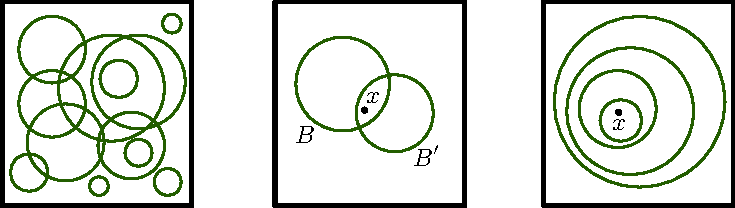
\includegraphics[width=3in]{ideas.pdf}
\end{center}
\caption{(a) A collection of balls $\B$. Ball $B$ has bias $\yh(B) \in \{-1,0,+1\}$. (b) If one ball has bias $+1$ and the other $-1$, points in their intersection are targeted for active querying. (c) Biases of progressively smaller balls containing $x$ might flip sign, leading to \emph{mind changes} about the label of $x$.}
\label{fig:challenges}
\end{figure}

There are three key challenges to be addressed. 

\begin{enumerate}
\item \label{challange:wheretoquery}
  {\bf Where to query?} \\
  Initial random querying tells us the biases of the largest balls,
  which gives some information about the decision boundary. In what
  parts of $\X$ might it be helpful to know biases of smaller balls,
  warranting further label queries? Our approach is simple: if a ball
  $B$ of bias $+1$ intersects a ball $B'$ of bias $-1$ then the
  intersection $B \cap B'$ is a ``known unknown'' and is targeted for
  active querying (Fig.~\ref{fig:challenges}(b)).

  This differs from the more conventional strategy of actively
  querying balls $B$ whose average $\eta$-value is close to zero. Such
  $B$ fall into two categories: (1) the $\eta$ values are close to
  zero throughout $B$, and (2) $B$ consists of two sub-regions, one
  strongly positive and the other strongly negative. In the first
  case, there is little merit in querying further. But in the second
  case, there is a lot to be gained. Our approach allows these two
  cases to be distinguished.

%To distinguish these two cases, we use a collection of balls that are \emph{overlapping}. For instance, we might take $\B$ to be \emph{all} balls in $\X$, which is effectively a finite collection once the given data points $X$ are taken into account. Case (2) can then be detected: we think of a point $x$ as being in the uncertainty region if it is contained in a ball $B$ that is strongly positive as well as being in a ball $B'$ that is strongly negative. Such points are ``known unknowns'', and these are the targets of our active querying.

\item \label{challange:nosmoothness}
  {\bf No smootheness assumptions}\\
  As no assumptions of smoothness are made, the sign of $\eta(\cdot)$
  can change in an arbitrarily small ball of any given point: the
  biases of balls containing $x$, say
  $B_1 \supset B_2 \supset \cdots$, might change sign a few times. At
  first, given only the bias of $B_1$, we might think $x$ has label
  $+1$. When we later estimate the bias of $B_2$, we could change our
  mind to $-1$. And then $+1$, and so on
  (Fig.~\ref{fig:challenges}(c)).


\item \label{challange:managingsampling}
  {\bf Managing sampling} \\
  The third challenge is \emph{managing sampling} of overlapping
  balls. We are interested in detecting points, and thus balls, whose
  $\eta$-values are either $> \gamma$ or $<-\gamma$. This suggests
  querying $k \approx 1/\gamma^2$ points at random from each
  ball. Now, suppose we have queried this many points from ball $B$
  and later want to query points from a different ball $B'$ that
  overlaps $B$. How can we reuse queries already made in $B \cap B'$?

\end{enumerate}

These three challenges go beyond earlier work in active learning, which was able to avoid problems like mind-changes by making smoothness assumptions on $\eta$. By tackling all three of them, we are able to give a
universal active learning scheme. 

The rest of the paper is organized as follows. Section~\ref{sec:relatedwork} describes related work.
Section~\ref{sec:algorithm} presents the active learning algorithm and Section~\ref{sec:discrete} analyzes it in generality, taking $X$ to be an arbitrary point-set and allowing any $\eta$ function. We identify two \emph{critical levels} for any $x \in X$: two scales (of ball sizes) that control how many queries are sufficient for $x$ to be correctly labeled (Theorem~\ref{thm:label-complexity}). We instantiate these bounds in canonical one-dimensional settings (Theorems~\ref{thm:oned-massart} and \ref{thm:oned-monotonic}) to get label complexities logarithmic in $|X|$.

Section~\ref{sec:continuous} considers the statistical setting where $X$ is drawn from an underlying distribution $\mu$ on $\X$. We give rates of convergence under distributional conditions (Theorem~\ref{thm:label-complexity-specific}), and instantiate them under common assumptions from learning theory and computational geometry.

\iffalse
\subsection{Results}

%Our algorithm does not require any assumption on the input distribution. In the worst case the number of queries is twice the number of queries of a passive algorithm. We show that under several natural conditions the query complexity of our algorithm is logarithmic in the error.


\fi


\subsection{Related work} \label{sec:relatedwork}

Existing work on non-parametric active learning yields algorithms that are guaranteed to work when the underlying conditional expectation $\eta(x)$ is smooth in some way. Additional assumptions are often needed.

This work can mostly be grouped by overall principle: either (1) they
seek to obtain the Bayes-optimal labels of a few well-positioned
points, and then propagate these to the rest of the space
\cite{DNZ15,H17,ASU18} or (2) they estimate the biases (positive or
negative) of entire regions at a time \cite{DH08,M12}. In this paper,
we follow the second strategy because the only reliable and
general-purpose way to assess the bias of an individual point,
$\mbox{sign}(\eta(x))$, is to query that point repeatedly; absent
smoothness assumptions, the sign can change abruptly in an arbitrarily
small ball around $x$. On the other hand, the bias of a region
$B$---the sign of the average $\eta$ value in $B$---is easy to
determine given a reasonable number of points from that region.

Early results of \cite{CN08} established upper and lower bounds on label complexity in situations where the Bayes-optimal boundary is of a simple form: a single threshold for one-dimensional data or a ``smooth boundary fragment'' in higher dimension.

An algorithm for active learning based on hierarchical sampling was given by \cite{DH08} and was analyzed under smoothness conditions by \cite{KUB15}. The idea is to begin with a hierarchical clustering of $X$, and to then use queries to discover a pruning of this tree whose leaf-clusters are almost-pure in their labels. The method is not well-suited to situations with significant noise levels. Another approach using dyadic partitions was given by \cite{M12} and analyzed under commonly-used smoothness, margin, and density assumptions---namely, that $\eta$ is Holder-smooth, the fraction of points with $|\eta(x)| \leq t$ is some polynomial in $t$, and the marginal density is close to uniform---along with an additional smoothness requirement on $\eta$.

A different strategy using nearest neighbors was explored by \cite{ASU18}. Their idea was to choose an appropriate scale $s$, find an $s$-cover of $X$, estimate the Bayes-optimal label for each point in this cover by querying its neighbors, and then use these cleanly-labeled points for 1-nearest neighbor classification. A somewhat more general approach was given by \cite{H17} and studied under the usual smoothness, margin, and density conditions, with resulting rates of convergence comparable to those found by \cite{M12}.

Finally, \cite{DNZ15} suggested a graph-based method for active learning based on adaptively looking for the cut in the graph corresponding to the correct decision boundary. Their assumptions are based on properties of this cut and are not easily comparable with earlier work.

The idea of predicting with balls of multiple sizes is a central theme of \cite{BDFM19}, which predicts at a point $x$ by choosing a ball centered at $x$ that is as small as possible while having a clear bias towards one label. That work does not consider active learning, which demands considerable further innovation. For instance, to assess the uncertainty at a point $x$, we need to look at balls containing $x$, not just those centered at $x$ (Fig.~\ref{fig:challenges}(b)).


Recall that the algorithm can query any $x \in X$ and receive $-1$ or $+1$ at random,
selected according to the conditional expectation function $\eta(x) = \E[y|x]$.

The goal of the algorithm is to make a small number of queries and then
assign Bayes-optimal labels to all points in $X$ with $|\eta(x)| \geq \gamma$.

The goal of our analysis is to characterize conditions under which the
number of queries is significantly smaller than
$\frac{|X|}{\gamma^2}\log \frac{1}{\gamma^2}$ which is the expected
  number of number of queries made by the naive algorithm that queries
  random elements of $X$ until each $x \in X$ has been sampled
  $\frac{1}{\gamma^2}$ times.

\section{Definitions}

The two basic entities in our algorithm are the collection of points
$X$ and a collection $\B$ of balls. Sampling is organized around a the
collection $\B$. Balls are the atomic sets on which we assess label
bias.

For any ball $B \in \B$, let $X_B = X \cap B$ be a shorthand for the
data points that lie in it.  We group balls into levels by the number
of points they contain. We put $B$ at {\it level} $\ell \geq 0$ if
\begin{equation}
\frac{|X|}{2^{\ell + 1}} \leq |X_B| < \frac{|X|}{2^\ell} .
\label{eq:sampling-level}
\end{equation}
Let $\B_\ell$ consist of all balls in $\B$ that are at level
$\ell$. Thus $\B_0, \B_1, \ldots$ is a partition of $\B$, with $\B_0$
consisting of highly-populated balls and subsequent
$\B_1, \B_2, \ldots$ consisting of successively smaller balls. We will
use $\B_{\geq \ell}$ to denote all balls at levels $\ell$ or greater,
and likewise $\B_{> \ell}$, $\B_{\leq \ell}$, and so on.

Balls in lower levels contain more points, and thus their biases
(average $\eta$ values) are easier to estimate. The main loop of the
simplified learning algorithm iterates over the levels $\ell=0,1,2,\ldots$

For any $x \in \X$, let $\B(x) \subset \B$ denote the collection of
balls that contain $x$ and can thus be used in determining $x$'s
label. We again partition these balls by sampling-level, so that
$\B_\ell(x) = \B(x) \cap \B_\ell$.

\section{A general-purpose active learning algorithm}
Our algorithm has several intricacies that might make it hard to
follow at a first read.  We therefor start with a description of a
simplified version of the algorithm (Fig~\ref{alg:siple}) that is not
completely correct but serves to explain the main components of the
detailed algorithm. The full description of the algorithm is given in
subsection~\ref{sec:full description} and appendix~\ref{sec:detailedalgorithm}

\begin{figure*}[t]
\framebox{
\begin{minipage}[t]{6in}  % Adjusted minipage width slightly
\begin{center}
\vspace{.1in}
\textbf{Repeat for $\ell=0,1,2,\ldots,\log |X|-1$:}
\begin{enumerate}[leftmargin=0.6cm]
\item \label{step:Uell} {\bf Compute uncertainty set:}\\ If $\ell=0$, set $U_0 = X$; otherwise set $U_\ell = \{x \in X: \yh_{\ell-1}(x) = \,!, \ \yh_\ell(x) = \bot\}$t
\item \label{step:QS} {\bf Compute Focused Query set:}\\ Compute query ball set be $R=  \bigcup_{x \in U} \B_\ell(x)$
and focused query set $S=\bigcup_{B \in R} B$
\item \label{step:sample} {\bf Make queries:}\\
\textbf{Repeat until} number of queries in each ball $B \in R$ is at least $C/\gamma^2$
  \begin{enumerate}[leftmargin=0.6cm]
  \item Select a {\tt query} uniformly at random from $S$
  \end{enumerate}

\item \label{step:balls} {\bf Update Ball labels:} For each ball $B \in R$, let $k(B)$ be
  the number of queries (of any kind) made inside $B$ and let
  $\widehat{\eta}(B)$ be the average of the labels returned by
  these queries.

  $$ \yh(B)
  =
  \left\{
    \begin{array}{ll}
%%%      \bot & \mbox{if $k(B) \leq \frac{C}{\gamma^2}$} \\
%%%      \sign(\widehat{\eta}(B)) & \mbox{if  $k(B) > \frac{C}{\gamma^2}$ and $|\widehat{\eta}(B)| \geq \gamma/2$} \\
      \sign(\widehat{\eta}(B)) & \mbox{if  $|\widehat{\eta}(B)| \geq \gamma/2$} \\
      0 & \mbox{otherwise}
    \end{array}
  \right.
  $$

\item \label{step:examples} {\bf Update example labels:} For each $x \in U_\ell$:
  \begin{align}
    \PL_\ell(x) &= \{s \in \{-1, +1\}: \ \text{there exists } B \in B_\ell(x) \text{ such that } \yh(B) = s \} \\ 
    \yh_\ell(x) &= 
                  \begin{cases}
                    +1 & \text{if } \PL_\ell(x) = \{+1\} \\
                    -1 & \text{if } \PL_\ell(x) = \{-1\} \\
                    0  & \text{if } \PL_\ell(x) = \{\} \\
                    !  & \text{if } \PL_\ell(x) = \{-1,+1\}
                  \end{cases}
                  \label{eq:provisional-label}
  \end{align}
\end{enumerate}
\end{center}

\end{minipage}}
\caption{A simplified version of the active learning algorithm.}
\label{alg:simple}
\end{figure*}

\subsection{Simplified algorithm}

We now describe the simplified algorithm here referred to simply as
the algorithm. The algorithm loops over increasing levels.  At each
level it identifies the set of ``known unknowns'' which approximates
the boundary. The algorithm then makes queries in the vicinity of the
boundary to refine it and proceeds to the next finer level.

What follows is a detailed explanation of  Figure~\ref{alg:simple}.

The outer loop of the algorithm iterates over the
levels, starting with $\ell=0$ that corresponds to balls that contain
at least half of the points in $X$, and ending with $\ell=\log |X|-1$,
corresponding to balls that contain a single point.

The loop consists of five steps. The first computes the uncertainty set, the second computes the focused query
set, the third defines the sampling process, the fourth and fifth
update the labels of the balls and the points respectively.

In step~\ref{step:Uell} the {\em uncertainty region} $U_\ell$ is
calculated. Intuitively $U_l$ is the set of points whose label
according to level $\ell-1$ is ! or ``known unknown'' and the label
according to level $\ell$ is $\bot$ or ``not enough information''.
These are the points for which we need better estimates.

In step~\ref{step:QS} the algorithm identifies the balls that needs to
be queried in order to get more information about $U_\ell$. These are
the balls in $\B_l$ that contain at least one point of $U_\ell$.  The
set $S$ is the union of these balls and defines the ``focus area''
which is queried in order to reduce the known unknowns.

In step~\ref{step:sample} the algorithm queries points inside the
focus area repeatedly at random.  This step terminates once there are
$C/\gamma^2$ samples in each of the balls in the focus area.

In step ~\ref{step:balls} associates a label with each ball. The
label is one of $\{-1,+1,0\}$.  The labels $+1$ and $-1$ correspond to
a confident statement that $\eta(B)>0$ and $\eta(B)<0$
respectively. Finally, the label $0$ indicates that the sign of $B$
is uncertain given the answers to the queries.

In step~\ref{step:examples} these labels are propagated to the
examples.  This is done in two sub-steps. First the {\em Possible
  Labels} for $x$ denoted $\PL_\ell(x)$ are calculated. $\PL_\ell(x)$
contains $+1$ if there is a ball containing $x$ whose label is $+1$,
symmetrically for $-1$. The label $\yh_\ell(x)$ is determined by the
possible labels set $\PL_\ell(x)$ as described in
step~\ref{step:examples}. The most significant label is ``!'', which
indicates balls with conflicting polarity containing $x$. Points
labeled ``!'' determine the uncertainty region and the focused query
region in the following level and the process repeats.


\iffalse
\subsection{Estimating the biases of balls}

The bias of a ball $B \in \B$ is defined as the average $\eta$ value in it,
$$ \eta_X(B) = \mbox{average}\{\eta(x): x \in X_B \} .$$
We estimate these biases using label queries and assign each ball a
\emph{qualitative} bias estimate $\yh(B)$,

Suppose that $k'$ queries have been made in the ball $B$ and let
$\widehat{\eta}(B)$ denote the mean of the answers to these queries.

step \ref{step:Uell} and \ref{step:QS} and \ref{step:balls} and \ref{step:sample} and \ref{step:examples}

We set the qualitative bias estimate as follows:
$$ \yh(B)
= 
\left\{
  \begin{array}{ll}
    \bot & \mbox{if $k \leq \frac{1}{\gamma^2}$} \\
\sign(\widehat{\eta}(B)) & \mbox{if  $k > \frac{1}{\gamma^2}$ and $|\widehat{\eta}(B)| \geq \gamma/2$} \\
0 & \mbox{otherwise}
\end{array}
\right.
$$

The option $\bot$ is used until enough points in $X_B$ have been queried: the required number is $k = O(1/\gamma^2)$ since $\gamma$ is the smallest bias that needs to be detected. Once this many labels are available, $\yh(B)$ is set to a value in $\{-1,0,+1\}$ and remains fixed thereafter.

These bias estimates will with high probability be seen to satisfy the following guarantee.
\begin{defn}
For any $B \in \B$, bias estimate $\yh(B) \in \{+1,-1,0\}$ is \emph{$\gamma$-accurate} if:
\begin{itemize}
\item $\yh(B) = +1 \implies \eta_X(B) > 0$
\item $\yh(B) = -1 \implies \eta_X(B) < 0$
\item $\yh(B) = 0 \implies |\eta_X(B)| < \gamma$
\end{itemize}
\label{def:accurate-bias-estimate}
\end{defn}

\subsection{Assigning labels to points}

The label of any point is inferred from the biases of balls containing it. 

Pick any $x \in X$ and any level $\ell$. Once qualitative bias estimates $\yh(B)$ are available for all balls at levels $\leq \ell$ that contain $x$ (that is, $\B_{\leq \ell}(x)$), we use these to infer a level-$\ell$ label for $x$. To begin with, the set of \emph{possible} labels for $x$ at level $\ell$, denoted $\PL_\ell(x) \subset \{-1,+1\}$, is defined thus:
\begin{itemize}[leftmargin=0.5cm]
\item $\PL_\ell(x)$ includes $+1$ if there exists a \emph{minimal} ball $B \in \B_{\leq \ell}(x)$ (with no other $B' \in \B_{\leq \ell}(x)$ strictly contained in it) for which $\yh(B) = +1$.
\item $\PL_\ell(x)$ includes $-1$ under a symmetrical condition.
\end{itemize}
This is made precise in Eqn~(\ref{eq:PL}) in Fig.~\ref{alg:main}. The label-estimate for $x$ at level $\ell$, denoted $\yh_\ell(x)$, is $+1$ if $\PL_\ell(x)=\{+1\}$, $-1$ if $\PL_\ell(x) = \{-1\}$, $0$ if $\PL_\ell(x) = \{\}$, and $!$ if $\PL_\ell(x) = \{-1,+1\}$ (Eqn~(\ref{eq:provisional-label})). 
%The interpretation of $\yh_\ell(x) \in \{+1,-1,0\}$ is given in Definition~\ref{def:accurate-bias-estimate}. 

The label $\yh_\ell(x) = \, !$ indicates that at level $\ell$, there is conflicting evidence about $x$; it is a ``known unknown''~\cite{R11}. Our active learning algorithm makes its \emph{focused queries} at level $\ell+1$ in the vicinity of such points $x$, that is, in $\B_{\ell+1}(x)$.

% to be $-1$ if $\PL_\ell(x) = %\{-1\}$, or $+1$ if $\PL_\ell(x) = \{+1\}$, or $0$ if $\PL_\ell(x) = \{\}$, or $!$ %if $\PL_\ell(x) = \{-1,+1\}$, %and remains fixed thereafter. Points labeled $!$ are ``known unknowns'': they are %near the decision boundary and %need further investigation. Points labeled $0$ show no significant bias.

\fi




\subsection{The detailed algorithm}
\label{sec:detailedalgorithm}

The simplified algorithm does addresses the first challange of ``where
to query'' (see challanges in the introduction). It does not address
the other two challanges, which the detailed algorithm does address.

\begin{enumerate}
\item {\bf No smoothness assumptions:}\\
  As described in the introduction, one can \emph{never} be sure of having
  correctly determined the label of $x$. Thus in addition to focused
  (active) querying, we also do background sampling of the entire
  space to pick up on possible mind changes. For simplicity, we make
  one background query per focused query.

  A related problem is that having the outer loop iterate over levels
  will cause the algorithm to miss some uncertainty region if they are
  appear at a lower level. Therefor the full algorithm does not loop
  over levels. Instead, at each iteration it finds the lowest level
  where the uncertainty set is not empty and makes two queries, one
  focused and one background.

\item {\bf Managing Sampling:}\\
  As described in the introduction, we would like to use queries that
  fall in the intersection of two balls for estimating the bias in
  both balls. However, selecting examples IID at random from the balls
  can create an undesired dependence between the estimates. This is solved using Poisson sampling, as described in section~\ref{sec:poisson}.
\end{enumerate}

\iffalse
We now describe the detailed active learning algorithm as shown in
Figs~\ref{alg:main}, \ref{alg:sampling} and~\ref{alg:bias-estimate}.
The algorithm makes two types of query. \emph{Background queries} are random draws
from $X$ and correspond to passive learning. \emph{Focused queries}
are made in the vicinity of ``uncertain'' points and correspond to
active learning.

Many of the elements of the detailed algorithm have been introduced in the simplified version.
Specifically $U_\ell,S,\PL_\ell(x),\yh_\ell(x)$, are as defined there.

However, in the detailed algorithm all of the levels are considered at each iteration.
On each iteration of the main loop (at most) one focused
query is made as well as a background query. The focused query comes
from the lowest-numbered uncertainty region $U_\ell$ that is nonempty.

Once these queries are made, bias estimates $\widehat{\eta}(B)$ are
updated using the Poisson method,\\
$\yh(B), \PL_\ell(x), \yh_\ell(x), U_\ell$ are updated
accordingly  and the next iteration begins.

The querying process can be stopped at any time, whereupon labels are assigned as follows:
\begin{equation}
\yh(x) = 
\left\{
\begin{array}{cl}
\yh_\ell(x) & \mbox{largest $\ell$ with $\yh_\ell(x) \in \{-1,+1\}$, if such an $\ell$ exists} \\
0 & \mbox{``don't know'', otherwise}
\end{array}
\right.
\label{eq:final-label}
\end{equation}

\begin{figure}[t]
\framebox{
\begin{minipage}[t]{6in}
\begin{center}
\begin{minipage}[t]{6in}
\vspace{.05in}

Initialize uncertainty regions at all levels: $U_0 = X$ and $U_\ell = \emptyset$ for $\ell \geq 1$

\vspace{.1in}

Initialize labels at all levels to ``unavailable'': \ $\yh_\ell(x) = \bot$ for all $x$ and $\ell \geq 0$

\vspace{.1in}

Repeat:
\begin{itemize}[leftmargin=0.5cm]
\item If there is a level $\ell \geq 0$ such that $U_\ell \neq \emptyset$:
\begin{itemize}[leftmargin=0.25cm]
\item For the smallest such level $\ell'$, run {\tt Focused-query}($\ell', U_{\ell'}$) // Fig.~\ref{alg:sampling}
\end{itemize}
\item Run {\tt Background-query} // Fig.~\ref{alg:sampling}
\item Update labels:
\begin{itemize}[leftmargin=0.25cm]
\item Update bias-estimates $\yh(B)$ // Fig.~\ref{alg:bias-estimate}
\item For each $x \in X$ and level $\ell \geq 0$ for which all $\{\yh(B): B \in \B_\ell(x)\}$ are available:
\begin{align}
\PL_\ell(x) &= \{s \in \{-1, +1\}: \ \mbox{there exists $B \in \B_{\leq \ell}(x)$ s.t. $\yh(B) = s$ and} \notag \\ 
             &                       \hspace{1.5in}\mbox{no $B' \in \B_{\leq \ell}(x)$ has $X_{B'} \subsetneq X_B$.} \} \label{eq:PL} \\ 
\yh_\ell(x) &= 
\left\{
\begin{array}{cl}
+1 & \mbox{if $\PL_\ell(x) = \{+1\}$} \\
-1 &  \mbox{if $\PL_\ell(x) = \{-1\}$} \\
0 & \mbox{if $\PL_\ell(x) = \{\}$} \\
! & \mbox{if $\PL_\ell(x) = \{-1,+1\}$}
\end{array}
\right.
\label{eq:provisional-label}
\end{align}

\end{itemize}
\item Update uncertainty regions:
\begin{itemize}[leftmargin=0.25cm]
\item $U_0 = \{x \in X: \yh_0(x) = \bot\}$
\item For all levels $\ell \geq 1$: \ $U_\ell = \{x \in X: \yh_{\ell-1}(x) = \,!, \ \yh_\ell(x) = \bot\}$
\end{itemize}
\end{itemize}

\end{minipage}
\end{center}
\end{minipage}}
\caption{The active learning algorithm. Each iteration of the main loop makes (at most) one focused query and one background query.}
\label{alg:main}
\end{figure}

\subsubsection{Poisson Sampling}
\label{sec:poisson}


The uncertainty region at level $\ell$ consists of the known-unknowns from level $\ell-1$, that is, points $x \in X$ with $\yh_{\ell-1}(x) = \, !$. This region is revealed to us piecemeal, a few points at a time. To get good label complexity we need to actively query the part of it we know.

We manage this through \emph{Poisson sampling} (Fig.~\ref{alg:sampling}). To infer the bias of a ball $B$, we need labels for $k = \tilde{O}(1/\gamma^2)$ random points in it. Balls at level $\ell$ have roughly $n/2^{\ell+1}$ points, so we need about $2^{\ell+1} k/n$ fraction of the ball to be queried. Instead, we query every point in the ball with probability $\tau_\ell = \min(2^{\ell+2}k/n, 1)$, \emph{independently}. Specifically, we query points $x$ in the ball with $T_x \leq \tau_\ell$, where each $x \in X$ is assigned a uniform-random value $T_x \in [0,1]$ at the outset of the algorithm. 

Once a point is queried, it is never queried again.

\begin{figure}[t]
\framebox{
\begin{minipage}[t]{6in}

\vspace{.05in}
\emph{Initialization:}
\begin{itemize}[leftmargin=0.5cm]
\item Set $Q = \emptyset$ (points queried so far)
\item For each $x \in X$: choose $T_x \sim \mbox{uniform}([0,1])$
\end{itemize}

\vspace{.05in}
{\bf Background-query}

\begin{itemize}[leftmargin=0.5cm]
\item Query the next unlabeled point in $X \setminus Q$, ordered by increasing $T_x$ values, and add to $Q$
\end{itemize}

\vspace{.05in}
{\bf Focused-query}($\ell, U$)

\begin{itemize}[leftmargin=0.5cm]
\item Define querying region:
$$ S =  \bigcup_{x \in U} \bigcup_{B \in \B_\ell(x)} \{z \in X_B: T_z \leq \tau_\ell\} $$
\item Query the next unlabeled point in $S \setminus Q$, ordered by increasing $T_x$ values, and add to $Q$
\end{itemize}

\end{minipage}}
\caption{The two sampling procedures. Each $x \in X$ has an associated r.v. $T_x$ drawn uniformly from $[0,1]$. The smaller $T_x$, the earlier $x$ is likely to be queried. \emph{Background queries} are drawn at random from $X$. \emph{Focused queries} are from the uncertainty region at a given level $\ell$, and use level-based thresholds $\tau_\ell = \min(2^{\ell+2}k/n, 1)$, where $k = \tilde{O}(1/\gamma^2)$.} 
\label{alg:sampling}
\end{figure}


\begin{figure}
\framebox{
\begin{minipage}[t]{6in}
\vspace{.05in}
\begin{itemize}[leftmargin=0.25cm]
\item Initially $\yh(B) = \bot$
\item When all of $\{z \in X_B: T_z \leq \tau_\ell\}$ is queried, let $\widehat{\eta}(B)$ be the mean of these labels and set
$$ \yh(B)
= 
\left\{
\begin{array}{ll}
\sign(\widehat{\eta}(B)) & \mbox{if $|\widehat{\eta}(B)| \geq \gamma/2$} \\
0 & \mbox{otherwise}
\end{array}
\right.
$$
\end{itemize}
\end{minipage}}
\caption{The qualitative bias $\yh(B)$ of a ball $B \in \B_\ell$; see Fig.~\ref{alg:sampling} for $\tau_\ell$.}
\label{alg:bias-estimate}
\end{figure}

\fi

\section{Analysis: finite population setting}
\label{sec:discrete}

We now analyze the active learning procedure in a setting where $X \subset \X$ is an arbitrary set of $n$ points. We make no distributional assumption on the manner in which $X$ is generated.

\subsection{Accuracy of bias estimates}

Fix the set of balls $\B$ and let $0 < \delta < 1$ be a
predefined confidence parameter. We start with a uniform guarantee on the
bias estimates for all balls $B \in \B$.

In Fig.~\ref{alg:sampling}, we see that the points queried in a ball $B$ at level $\ell$ are $\{z \in X_B: T_z \leq \tau_\ell\}$, which from the definition of $\tau_\ell$ has size $O(k)$. We use these labels to estimate the bias of $B$. Since we need to detect biases of magnitude greater than $\gamma$, we set $k \propto 1/\gamma^2$. 
%This intuition is borne out by the following result, proved in the appendix. 
\begin{lemma}
Suppose that $k \geq (192/\gamma^2) \ln (4 |\B|/\delta)$. 
Let $\yh(B)$ be defined as in Fig.~\ref{alg:bias-estimate}. Then with probability $\geq 1-\delta$, all the $\yh(B)$, for $B \in \B$, are $\gamma$-accurate in the sense of Definition~\ref{def:accurate-bias-estimate}.
\label{lemma:accurate-bias-estimates}
\end{lemma}
Henceforth assume $\yh(B)$ is $\gamma$-accurate for all  $B \in \B$.


\subsection{Critical levels}

Recall that $\PL_\ell(x) \subset \{-1,+1\}$ denotes the possible labels for $x$ given information from balls at levels $\leq \ell$, and is used to assign a value $\yh_\ell(x) \in \{-1,+1,0,!\}$. Despite randomness in querying, it is possible to define two critical levels for each $x$: a level $L_1(x)$ by which $\PL_\ell(x)$ reliably contains the correct label of $x$, and a level $L_2(x)$ by which $\PL_\ell(x)$ reliably omits the wrong label.

\begin{defn}[Critical levels $L_1,L_2$]
Pick any $x \in X$ with $\eta(x) \neq 0$ and let $s(x) = \sign(\eta(x))$. Define $L_1(x)$ to be the smallest level $\ell$ such that there exists $B_o \in \B_\ell(x)$ for which
\begin{itemize}[leftmargin=0.5cm]
\item $s(x) \cdot \eta_X(B_o) \geq \gamma$, and
\item $s(x) \cdot \eta_X(B) \geq \gamma$ for any $B \in \B(x)$ with $X_{B} \subset X_{B_o}$.
\end{itemize}
Define $L_2(x)$ to be the smallest level $\ell$ such that:
\begin{itemize}[leftmargin=0.5cm]
\item For all $B \in \B_{\geq \ell}(x)$, we have $s(x) \cdot \eta_X(B) \geq 0$.
\item For any $B \in \B_{\leq \ell}(x)$ with $s(x) \cdot \eta_X(B) < 0$, there exists $B' \in \B_{\leq \ell}(x)$ with $X_{B'} \subset X_B$ and $s(x) \cdot \eta_X(B') \geq 0$.
\end{itemize}
Take $L_1(x)$ or $L_2(x)$ to be $\infty$ if no level meets the requirements, or if $\eta(x) = 0$. 
\label{defn:L12}
\end{defn}

Once $\ell$ reaches a critical level, $\PL_\ell(x)$ and thus $\yh_\ell(x)$ behave more predictably, as follows.
\begin{lemma}
Pick any $x \in X$ with $\eta(x) \neq 0$ and let $s(x) \in \{+1,-1\}$ denote its Bayes-optimal label. Then for any level $\ell$ and any time at which $\yh_\ell(x) \neq \bot$:
\begin{enumerate}
\item[(a)] If $\ell \geq L_1(x)$, then $s(x) \in \PL_\ell(x)$ and thus $\yh_\ell(x) \in \{s(x), !\}$. 
\item[(b)] If $\ell \geq L_2(x)$, then $-s(x) \not\in \PL_\ell(x)$ and thus $\yh_\ell(x) \in \{s(x), 0\}$.
\end{enumerate}
\label{lemma:boundary}
\end{lemma}

\subsection{Boundary sets and label complexity}

A common intuition about active learning is that successive queries gradually constrain the possible locations of the decision boundary. Let's consider the state of affairs when all balls at level $\leq \ell - 1$ have been sampled. The known-unknowns from this level are points $x$ with $\yh_{\ell-1}(x) = \, !$; by Lemma~\ref{lemma:boundary}(b), such points must have $L_2(x) \geq \ell$. Focused sampling at level $\ell$ is restricted to balls that contain these points. We will think of this region as the \emph{boundary set} at level $\ell$.
\begin{defn}[Boundary set $\bf \Delta_\ell$]
For any level $\ell$, define the \emph{boundary set} at level $\ell$ to be
\begin{equation}
\Delta_\ell 
= \bigcup_{x \in X: L_2(x) \geq \ell} \bigcup_{B \in \B_{\ell}(x)} X_B 
.
\label{eq:sampling-region}
\end{equation}
\end{defn}
%It can be shown that all focused samples at level $\ell$ must lie in this set.
\begin{lemma}
All focused samples at level $\ell$ lie in $\{z \in \Delta_\ell: T_z \leq \tau_\ell \}$.
\label{lemma:focused}
\end{lemma}

We can now give generic label complexity bounds in terms of $L_1$, $L_2$, and $\Delta_\ell$. These take two equivalent forms: a \emph{global} version that specifies what parts of $X$ are correctly labeled after $m$ queries and a \emph{local} version that specifies the number of queries after which a particular $x$ is correctly labeled. The global version (Theorem~\ref{thm:label-complexity-0}) is in the Appendix; here is the local version.

\begin{thm}[Local query complexity]
Take $k \geq (192/\gamma^2) \ln (4 |\B|/\delta)$. With probability at least $1-2\delta$, the following holds simultaneously for all $x \in X$. Let $L_1(x)$ and $L_2(x)$ be the critical levels for $x$, as in Definition~\ref{defn:L12}. If $L_2(x) \leq \lg (n/2k)$, let
\[
m_o(x) = 32k \cdot \max\bigg( 2^{L_1(x)}, \ \frac{1}{n} \sum_{\ell=L_1(x)+1}^{L_2(x)} |\Delta_\ell| \, 2^\ell\bigg) .
\]
Once the active learner has made $m_o(x)$ queries, $\yh(x)$ is fixed at the Bayes-optimal label $g^*(x)$.
\label{thm:label-complexity}
\end{thm}
Let's interpret this bound. For a specific $x \in X$, there is no telling how $\yh_\ell(x)$ will behave at levels $\ell < L_1(x)$. But for $\ell \geq L_1(x)$, either $\yh_\ell(x) = \, !$, in which case $x$ is in the uncertainty region, or the label of $x$ is correctly set once and for all, which occurs by level $L_2(x)$. 

We will say that $x$ \emph{reaches level $\ell$} when bias estimates have been obtained for all balls in $\B_{\leq \ell}(x)$ and thus $\yh_\ell(x)$ is set. Recalling that the algorithm alternates between background and focused queries, we show that $m_o(x)/4$ \emph{background} queries suffice for $x$ to reach level $L_1(x)$ and an additional $m_o(x)/4$ \emph{focused} queries take it to level $L_2(x)$, by which time its label is correct.

In particular, $O(k \cdot 2^\ell)$ background queries give us the biases of all balls in $\B_{\leq \ell}$; this is the first term in $m_o(x)$. And there are $O(k \cdot 2^\ell \cdot |\Delta_\ell|/n)$ focused queries at any level $\ell$: the second term.

A footnote: Our algorithm queries points at most once. However, in some applications, a point $x$ can be queried repeatedly, each time producing an independent draw from $\eta(x)$. If \emph{repeat queries} are permissible, $O(1/\gamma^2)$ copies should be made of each point in $X$ before the algorithm is applied; and in this case, points with $|\eta(x)| \geq \gamma$ will all be correctly labeled, eventually.



\section{One-dimensional examples}

To apply Theorem~\ref{thm:label-complexity}, we need bounds on the critical levels $L_1(x)$ and $L_2(x)$ for each $x \in X$, and on the size of the sampling region $\Delta_\ell$ at each level $\ell$. We now derive these in some canonical settings.

\begin{figure}
\begin{center}
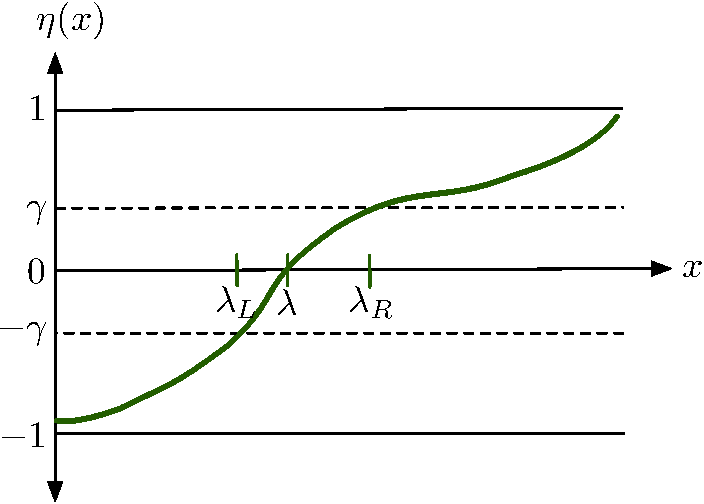
\includegraphics[width=2.5in]{oned-monotonic.pdf}
%\hspace{.5in}
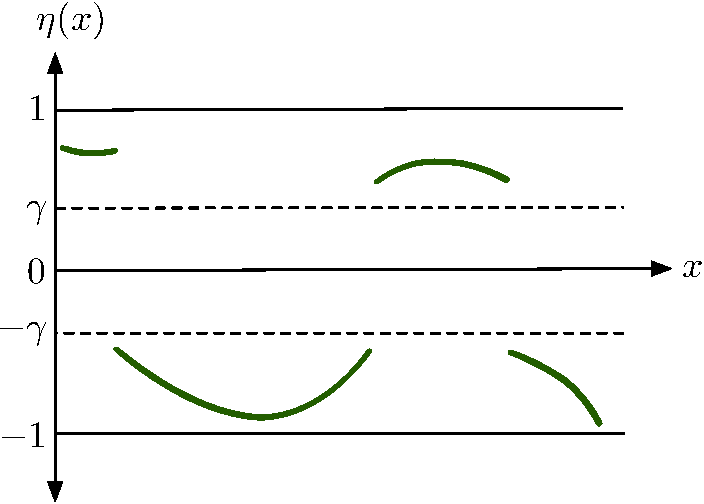
\includegraphics[width=2.5in]{oned-massart.pdf}
\end{center}
\caption{(a) The conditional probability function $\eta$ is monotonically increasing; $\eta(x) = -\gamma, 0, \gamma$ at $x = \lambda_L, \lambda, \lambda_R$, respectively. (b) On each subinterval, $\eta$ is either $> \gamma$ or $<-\gamma$.}
\label{fig:oned}
\end{figure}

\subsection{Example: monotonic $\eta$}

Suppose $X$ is an arbitrary set of $n$ points in $\X = [0,1]$ and is labeled according to a conditional probability function $\eta: \X \to [-1,1]$ that is continuous and strictly increasing (Fig.~\ref{fig:oned}(a)). Let $\lambda \in (0,1)$ be the point for which $\eta(\lambda) = 0$ and let $\lambda_L, \lambda_R$ be the points for which $\eta(\lambda_L) = -\gamma$ and $\eta(\lambda_R) = \gamma$. Thus we are not required to label points in the interval $(\lambda_L, \lambda_R)$. 




%\begin{figure}
%\begin{center}
%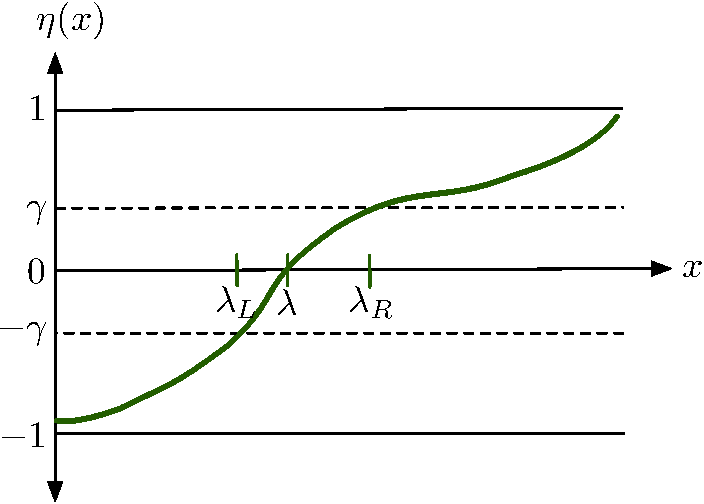
\includegraphics[width=3in]{oned-monotonic.pdf}
%\end{center}
%\caption{The conditional probability function $\eta$ is monotonically increasing. The values $x = %\lambda_L, \lambda, \lambda_R$ have $\eta(x) = -\gamma, 0, \gamma$ respectively.}
%\label{fig:oned-monotonic}
%\end{figure}


Let $\B$ consist of all closed intervals. Although there are infinitely many of these, we need only consider those whose endpoints lie in $X$, so effectively $|\B| = O(n^2)$.

The critical levels are easy to bound in this setting. Let $n^- = |[0,\lambda_L] \cap X|$  be the number of points to the left of $\lambda_L$ and $n^+ = |[\lambda_R,1] \cap X|$ the number of points to the right of $\lambda_R$. Then 
%\begin{align*}
%L_1(x)
%&\leq
%\left\{
%\begin{array}{ll}
%\lg (n/n^+) & \mbox{if $x \geq \lambda_R$} \\
%\lg (n/n^-) & \mbox{if $x \leq \lambda_L$}
%\end{array}
%\right.
%\\
%L_2(x)
%&\leq
%\lg (n/r(x))
%\end{align*}
$$
L_1(x)
\leq
\left\{
\begin{array}{ll}
\lg (n/n^+) & \mbox{if $x \geq \lambda_R$} \\
\lg (n/n^-) & \mbox{if $x \leq \lambda_L$}
\end{array}
\right.
\mbox{\ \ \ \ and \ \ \ }
L_2(x)
\leq
\lg (n/r(x))
$$
where $r(x)$ is the number of data points between $x$ and $\lambda$, counting $x$ as well.
%\begin{itemize}
%\item $L_1(x) \leq \lg (n/n^+)$ if $x \geq \lambda_R$ and $L_1(x) \leq \lg (n/n^-)$ if %$x \leq \lambda_L$, and
%\item $L_2(x) \leq \lg (n/r(x))$, 
%\end{itemize}

A counting argument then shows that the boundary region shrinks exponentially as the level increases, $|\Delta_\ell| \leq 4n/2^\ell$, yielding the following label complexity. 
\begin{thm}
Define $r^+ = \min \{r(x): x \in X \cap [\lambda_R,1]\}$ and $r^- = \min \{r(x): x \in X \cap [0,\lambda_L]\}$. Pick any $0 < \delta < 1$. Suppose we run the algorithm of Fig.~\ref{alg:main} with $k = O((\log (n/\delta))/\gamma^2)$ and that $\min(r^+, r^-) \geq 2k$.  Take any 
$$ m \geq 64k \cdot \max \left( \frac{n}{\min(n^+,n^-)}, \ 2 \lg \frac{\min(n^+,n^-)}{\min(r^+,r^-)} \right) .$$
With probability $\geq 1-\delta$, after $m$ queries the algorithm correctly labels all $x \in X$ with $|\eta(x)| \geq \gamma$.
\label{thm:oned-monotonic}
\end{thm}
If $n^+, n^- = \Theta(n)$, that is, a constant fraction of the points lie to the left of $\lambda_L$ and to the right of $\lambda_R$, then the label complexity is $O(\log^2 n)$. If in addition $r^+, r^- = \Theta(n)$, that is, a constant fraction of the points lie between $\lambda_L, \lambda_R$ and the decision boundary, the label complexity is $O(\log n)$. 

\subsection{Example: Massart noise}

In Section~\ref{sec:oned-massart}, we develop another one-dimensional example, in which $\X$ consists of several pieces, such that on each piece $\eta$ is either entirely above $\gamma$ or entirely below $-\gamma$ (Fig.~\ref{fig:oned}(b)). Once again, a logarithmic label complexity is obtained.


\section{Analysis: distributional setting}
\label{sec:continuous}

We now turn to a setting where the points $X$ are drawn from some distribution $\mu$ on a topological space $\X$. For the same algorithm, we bound label complexity in terms of properties of $\mu$ and $\eta$. 

\subsection{A sufficiently-rich collection of balls}

Let $\B$ be a finite collection of subsets of $\X$; we spell out a basic property we need it to possess.

\begin{defn}
We say $\B$ is \emph{$k$-conforming} with respect to $X$ if 
\begin{itemize}
\item ({\bf Richness}) For any $x \in X$, there exists $B \in \B_0(x)$. Moreover, for any level $0 \leq \ell \leq \lg (n/k)$ and any $B \in \B_\ell(x)$, there exists $B' \in \B_{\ell+1}(x)$ such that $X_{B'} \subset X_B$.
\item ({\bf Fidelity}) $\mu(B)/2 \leq |X_B|/n \leq 2\mu(B)$ for all $B \in \B$ with $|X_B| \geq k$.
\end{itemize}
\label{defn:conformity}
\end{defn}
When $\B$ consists of Euclidean balls in $\R^d$, made finite by restricting to $X$, the first property is immediate and the second holds with high probability (Lemma~\ref{lemma:ball-size-bounds}). We also envisage scenarios where $\B$ is constructed using $X$, for instance from the cells of multiple spatial partition trees.

Henceforth assume $\B$ satisfies this property.  We ignore $B$ with $|X_B| < k$, thereby restricting attention to levels $0 \leq \ell < \lg (n/k)$.

\subsection{A probabilistic notion of distance}

A crucial step in the analysis is to introduce a distance function based on $\mu$: the distance from a point $x$ to a set $S$ is the probability mass of the smallest ball that contains $x$ and touches $S$.
\begin{defn}
For any $x \in \X$ and $S \subset \X$, define
$\dist(x,S) = \inf \{\mu(B): B \in \B(x), B \cap S \neq \emptyset\} .$
\label{defn:prob-dist}
\end{defn}
We will see that $L_2(x)$ can be bounded in terms of such distances. In what follows, for $s \in \{-1,0,+1\}$, take $\X^s$ to denote $\{x \in \X: \sign(\eta(x)) = s\}$.
\begin{lemma}
For any $x \in \X$, let $s(x) = \sign(\eta(x))$. If $\dist(x, \X^{-s(x)}) \geq 2k/n$, then
$L_2(x) \leq \bigg\lceil \lg \frac{1}{\dist(x, \X^{-s(x)})} \bigg\rceil + 1$.
\label{lemma:L2-bound}
\end{lemma}
We will also use probabilistic distance to define notions of boundary. Take the $p$-boundary to consist of points at distance $\leq p$ from points of the opposite label.
\begin{defn}
For any $p > 0$, define $\partial_p = \{x \in \X: \dist(x, \X^{-s(x)}) \leq p\}$.
\label{defn:boundary}
\end{defn}
This includes all $x$ with $\eta(x) = 0$. Next, the $(p,q)$-boundary consists of points at distance $\leq q$ from the $p$-boundary.
\begin{defn}
For any $p,q > 0$, define $\partial_{p,q} = \{x \in \X: \dist(x, \partial_p) \leq q\}$.
\label{defn:boundary2}
\end{defn}

We can bound $\Delta_\ell$, the query region at level $\ell$, in terms of this second-order boundary.
\begin{lemma}
For any $0 \leq \ell \leq \lg (2n/k)$, we have $\Delta_\ell \subset \partial_{4/2^\ell, 2/2^\ell}$.
\label{lemma:delta-continuous}
\end{lemma}
Theorem~\ref{thm:label-complexity} thus still holds with $n \cdot \mu(\partial_{4/2^\ell, 2/2^\ell})$ in place of $|\Delta_\ell|$; see Theorem~\ref{thm:label-complexity-dist} in the Appendix. 

Using these notions, we are able to specialize the generic label complexity bound of Theorem~\ref{thm:label-complexity} to get rates under suitable margin conditions; this is given in Theorem~\ref{thm:label-complexity-specific} in the appendix. Here we just give a concrete scenario handled by the latter result; another such scenario, with smoothness and Tsybakov noise conditions, appears in the appendix.

%\begin{figure}[t]
%\begin{center}
%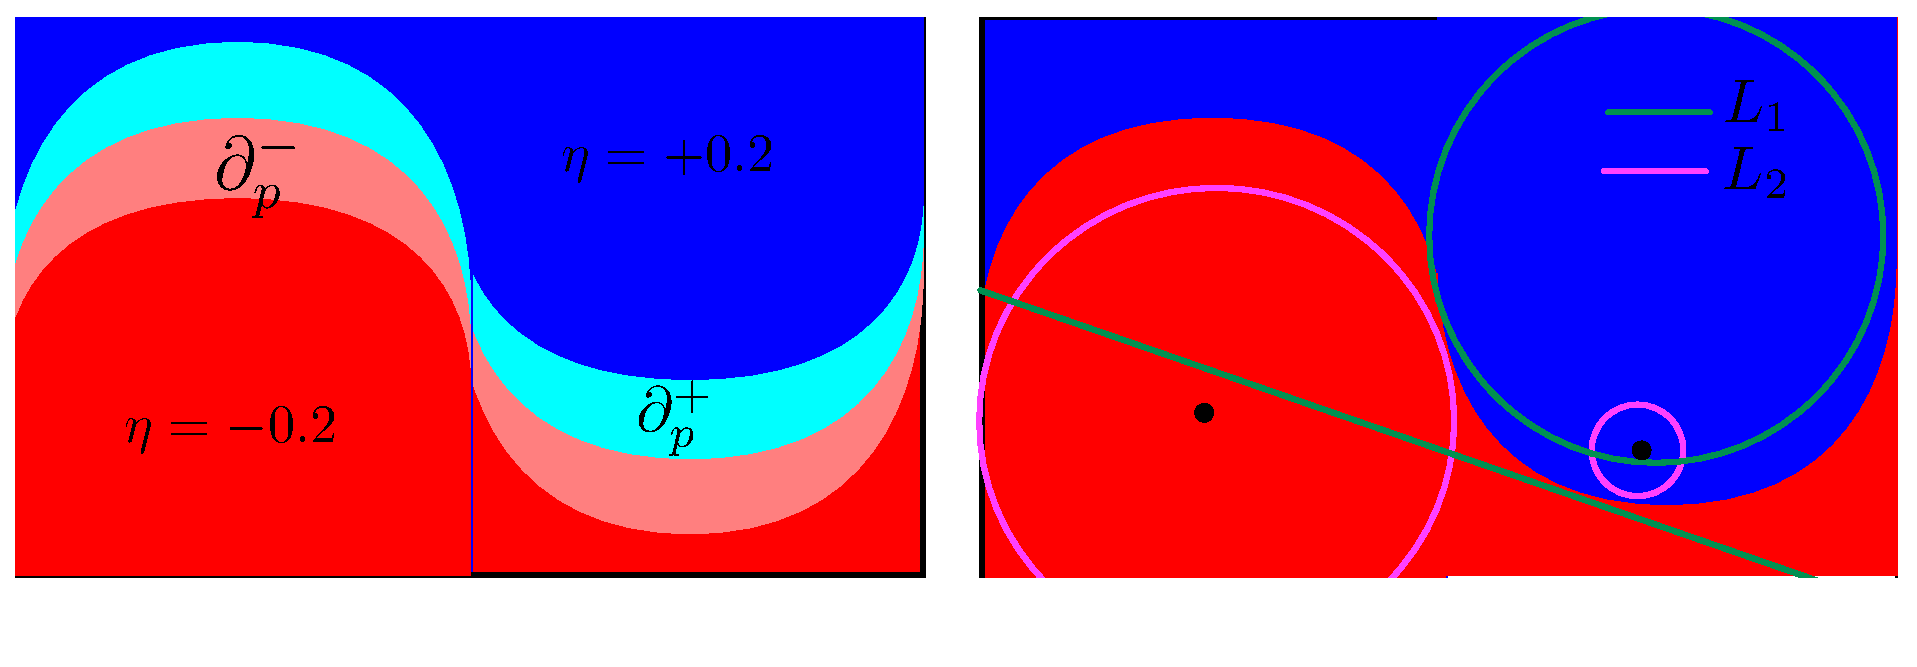
\includegraphics[width=3in]{curvature.pdf}
%\end{center}
%\caption{{\bf A 2D example with bounded curvature:} {\em Left:} We have $\eta = -0.2$ for the orange/red part of the domain and $\eta=0.2$ for the light and dark blue. The orange and light blue indicate the boundary sets for negative and positive respectively. {\em Right:} examples of the $L_1,L_2$ balls for different points. The green $L_1$ circles are the largest monochrome circle that contains the point. The purple $L_2$ circles are the union of all circles of half the radius or smaller. All of these circles are monochrome.}
%\label{fig:curvature}
%\end{figure}


\subsection{Example: Curvature and Massart noise}
\label{sec:Massart}

By way of example, consider a case where $\X \subset \R^d$ and $\mu$ admits a density. We take $\B$ to consist of all open balls $B(x,r) = \{z: \|z-x\| < r\}$ centered in $\X$, with $\B(x)$ being balls that contain $x$. By VC arguments, the size of $\B$ is effectively $O(n^{d+1})$; in practice, this can be reduced to a low-order polynomial using core-sets~\cite{BC03}.

We make two key assumptions: distribution $\mu$ on $\X$ is within a multiplicative factor of uniform; and all of $\X$ has $|\eta(x)| \geq \gamma$ except for a $(d-1)$-dimensional boundary of finite curvature.
\begin{itemize}[leftmargin=0.5cm]
\item (Strong density condition)
There are constants $c_o, c_1 > 0$ such that for all balls $B \in \B$,
we have $c_o \vol(B) \leq \mu(B) \leq c_1 \vol(B) $, where $\vol(\cdot)$ is $d$-dimensional volume.
\item (Massart noise and boundary condition) $\X = \X^+ \cup \X^- \cup \X^0$, where: $\eta(x) \geq \gamma$ throughout $\X^+$; $\eta(x) \leq -\gamma$ throughout $\X^-$; and $\X^0$ separates (intersects any line between) $\X^+$ and $\X^-$ and is a $(d-1)$-dimensional Riemannian manifold of reach $r_o > 0$.
\end{itemize}
The \emph{reach} condition says that any point at distance $< r_o$ of $\X^0$ has a unique nearest neighbor on $\X^0$. It is a common notion of curvature~\cite{F59,NSW06} and implies that $\X^+$ (resp., $\X^-$) can be covered by open balls of radius $r_o$ that do not touch $\X^- \cup \X^0$ (resp., $\X^+ \cup \X^0$). A 2D example obeying these conditions appears in Figure~\ref{fig:curvature}.
\begin{thm}
  Under the two conditions above, there are constants $c_2, c_3$ for
  which the following holds. Pick $0 < \delta < 1$ and take
  $k = O(((d \log n) + \log (1/\delta))/\gamma^2)$. If the algorithm
  of Fig.~\ref{alg:main} makes $c_2k \leq m \leq c_3 n^{(d-1)/d}$
  queries, it assigns Bayes-optimal labels to all but
  $C (k/m)^{1/(d-1)} + (2/n) \log (4/\delta)$ fraction of $X$.
\label{thm:massart-dist}
\end{thm}

 Here the constant $c_2$ includes a term $(1/r_o)^d$. The
$\tilde{O}(1/m^{1/(d-1)})$ rate of this theorem is an improvement over
the usual $1/m^{1/d}$ rate for random querying and was also observed
earlier, in a more restricted setting, using specialized
algorithms~\cite{CN08}.

%\documentclass{article}
\usepackage{fullpage}
\usepackage{amsmath,amssymb,amsfonts}
\usepackage{graphicx}
\usepackage{natbib}

\def\R{{\mathbb{R}}}
\def\pr{{\rm Pr}}
\def\E{{\mathbb E}}
\def\X{{\mathcal X}}
\def\Y{{\mathcal Y}}
\def\H{{\mathcal H}}
\def\G{{\mathcal G}}
\def\B{{\mathcal B}}
\def\bias{{\rm bias}}
\def\supp{{\rm supp}}

\newtheorem{thm}{Theorem}
\newtheorem{lemma}[thm]{Lemma}
\newtheorem{cor}[thm]{Corollary}
\newtheorem{claim}[thm]{Claim}
\newtheorem{defn}[thm]{Definition}
\newtheorem{assump}{Assumption}
\newtheorem{open}{Open problem}
\newenvironment{proof}{\noindent {\sc Proof:}}{$\Box$ \medskip}

\DeclareMathOperator*{\argmax}{arg\,max}

\title{An active $k$-nearest neighbor algorithm}

\begin{document}

\maketitle

\section{Setup}

Basic Transductive setup:
\begin{itemize}
\item Intance set $\X =\{x_1,\dots,x_n\}$, $x_i in \R^d$. The set $\X$
  is fixed and known to the learner. The probability of each $x \in
  \R$ is $1/n$. 
\item Label space $\Y = \{-1,+1\}$. Each $x \in \X$ is associated with
  a conditional probability function $\eta(x) = \pr(Y=1|X=x)$.
\item Let $g^*$ denote the Bayes-optimal classifier on $\X$:
  $$ g^*(x) = \mbox{sign}(2 \eta(x) - 1) .$$
  \item Label Queries: the algorithm can select any example $x \in
    \X$, as a response it gets a label in $\Y$ chosesn acccording to
    $\eta(x)$.    
  \end{itemize}

\section{Notation}
\begin{itemize}
  \item {\bf Balls:} $B(x,r)$ denotes a ball of radius $r$ centered at $x$.
  \item {\bf Probability of a ball} The probability of a ball is the
    fraction of points in $\X$ that fall inside $B(x,r)$.
    $$ \mu(B(x,r)) = \frac{ |B(x,r) \cap \X|}{n} $$
  \item {\bf measuring radius in terms of probability}
For any $x \in X$ and any $p > 0$, let $r_p(x)$ denote the smallest radius $r$ such that $\mu(B(x, r)) \geq p$. 
\end{itemize}

For any $p, \gamma> 0$, let $\X_{p, \gamma}$ consist of all points $x \in \supp(\mu)$ such that:
\begin{itemize}
\item either $\eta(B(x,r)) \geq 1/2 + \gamma$ for all $0 \leq r \leq r_p(x)$ 
\item or $\eta(B(x,r)) \leq 1/2 - \gamma$ for all $0 \leq r \leq r_p(x)$.
\end{itemize}


\section{Algorithm for pool-based active learning}

Global variables:
\begin{itemize}
\item $U \subset X$, a subset of points deemed ``uncertain''
\item $Q \subset X$, points whose labels have been queried
\item $R \subset Q$, points in $Q$ that are random draws from the entire space $X$
\item $I \subset X$, points whose labels have been inferred, possibly incorrectly
\end{itemize}

We will use large deviation bounds for the class $\B$ of balls centered at points of $X$. This is a class of size at most ${n \choose 2}$. The bounds will assert the following: suppose $m$ points are drawn i.i.d. from $\mu|_S$, the restriction of $\mu$ to a subset $S \subset \X$, and labeled according to $\eta$. Then with probability at least $1-\delta$, the following properties hold for all $B \in \B$:
\begin{enumerate}
\item[(P1)] If $\mu|_S(B) \geq (k/m) \ln (n/\delta)$, then $B$ gets at least $k+1$ points.
\item[(P2)] If $B$ gets at least $k$ points, then the average of the labels in $B$ is equal to $\eta(B) \pm k^{-1/2}$.
\end{enumerate}
We will use several rounds of sampling. Let $G_t$ denote the good event that these conditions hold for the points drawn in round $t$.

\subsection{A single round of sampling}

\begin{figure}[h!]
\framebox{
\begin{minipage}[t]{6.3in}
{\bf function Extend}($k$, $p$, $\delta$):
\begin{itemize}
\item Setup:
\begin{itemize}
\item Define the region of uncertainty:
$$ U = X \setminus (Q \cup I) $$
\item Determine the sampling region:
$$ S =  \left( \bigcup_{x \in U} B(x, r_p(x)) \right) \cap X $$
\item Choose number of samples:
$$ m = \frac{|S|}{|X|} \cdot \frac{k}{p} \cdot \ln \frac{n}{\delta} $$
\end{itemize}

\item Querying:
\begin{itemize}
\item Let $M$ consist of $m$ points chosen uniformly at random from $S$
\item Let $M'$ consist of $m$ points chosen uniformly at random from $X$
\item For all $x \in (M \cup M') \setminus Q$: 
\begin{itemize}
\item Query $x$'s label
\item Add $x$ to $Q$
\end{itemize}
\item $R = R \cup M'$
\end{itemize}

\item Update:
\begin{itemize}
\item For all $x \in U$:
\begin{itemize}
\item Find the $k$ nearest neighbors of $x$ in $M$ (can probably do $M \cup R$)
\item If their labels have significant bias, in the sense that their average has absolute value $\geq k^{-1/2}$, label $x$ accordingly and add it to $I$
\end{itemize}
\item For all $x \in I$:
\begin{itemize}
\item Find the $k$ nearest neighbors of $x$ in $R$
\item If their labels have significant bias and disagree with $x$'s current label, move all of $B(x,r_p(x)) \cap (I \setminus \{x\})$ out of $I$ (not sure exactly what to do here)
\end{itemize}
\end{itemize}
\end{itemize}
\end{minipage}}
\caption{Extend: the key subroutine for pool-based active learning}
\label{fig:extend}
\end{figure}

\begin{lemma}
Consider round $t$ of sampling. Suppose event $G_t$ holds. For any $x$, let $\widetilde{r}(x)$ denote the smallest radius $r$ such that $B(x,r)$ contains $k+1$ points of $M$. Then for all $x \in U$,
\begin{enumerate}
\item[(a)] $\widetilde{r}(x) \leq r_p(x)$
\item[(b)] the bias of the $k$ nearest neighbors of $x$ in $M$ agrees with $\eta(B(x,\widetilde{r}(x))) \pm 1/k^{1/2}$.
\end{enumerate}
\label{lemma:bias-bound}
\end{lemma}
\begin{proof}
Let's begin with (a). Choose any $x \in U$ and write $B = B(x,r_p(x))$. The points in $M$ can be considered to be $m$ i.i.d. draws from $\mu|_S$. Ignoring the small discrepancy between $\mu(S)$ and $|S|/|X|$, we have 
$$ \mu|_S(B) = \frac{\mu(B)}{\mu(S)} \geq \frac{p}{\mu(S)} \geq \frac{k}{m} \ln \frac{n}{\delta}$$
and thus by (P1) $M$ includes at least $k+1$ points of $B$.

Part (b) then follows directly by appealing to (P2).
\end{proof}

\begin{thm}
Suppose that in round $t$, the starting uncertainty region is $U$. Assume event $G_t$ occurs. Then for all $x \in U$ that aren't queried, the following two properties hold.
\begin{enumerate}
\item[(a)] If $x \in \X_{p, 2k^{-1/2}}$, then by the end of the round, its label is inferred to be $g^*(x)$.
\item[(b)] If the label of $x$ is inferred but is not equal to $g^*(x)$, then $x \not\in \X_{p, k^{-1/2}}$.
\end{enumerate}
\end{thm}
\begin{proof}
Pick any $x \in U$ whose label is not queried by the end of round $t$. By Lemma~\ref{lemma:bias-bound}, its $k$ nearest neighbors in $M$ lie within distance $\widetilde{r}(x) \leq r_p(x)$, and its $k$ nearest neighbors have average label in the range $\eta(B(x, \widetilde{r}(x))) \pm k^{-1/2}$. 

For part (a), observe that by the definition of $\X_{p,\gamma}$, this average label has sign $g^*(x)$ and absolute value $> k^{-1/2}$. Thus the bias is significant and the label of $x$ is correctly inferred.

For part (b), we observe that if $x \in \X_{p, k^{-1/2}}$, then the average label of $x$'s $k$ nearest neighbors would have the correct sign, $g^*(x)$.
\end{proof}

\subsection{A simple active learning loop}

Here's a simple idea: keep $k$ fixed, with the goal of trying to correctly classify all $x \in \X_{p,\gamma}$ with $p > 1/n$ and $\gamma > 1/\sqrt{k}$. We won't quite be able to do this because of mind-changes.

\begin{itemize}
\item Given: $X$, $\gamma$, $\delta$
\item $k = 1/\gamma^2$
\item $Q = I = \emptyset$
\item for $t = 0, 1, \ldots, \log n$:
\begin{itemize}
\item $p_t = 1/c^t$
\item $\delta_t = \delta/(1 + \log n)$
\item Extend($k$, $p_t$, $\delta_t$)
\end{itemize}
\end{itemize}

Let's start by analyzing this in the case where there are no mind-changes.

\subsection{Analysis: no mind changes}

Fix $\gamma = k^{-1/2}$. For $\tilde{p} \sim 1/n$, define $\widetilde{\X}^+ = \X_{\tilde{p}, \gamma}$ and likewise $\widetilde{\X}^-$. Then $\widetilde{\X} = \widetilde{\X}^+ \cup \widetilde{\X}^-$ is exactly the set of points that could reasonably be expected to be correctly classified by a $k$-NN classifier with access to all the labels in $X$. We'd like to do almost as well after querying just a fraction of the labels.

\begin{enumerate}
\item {\it No mind changes.} We will assume no mind-changes: that is, for any $r>0$,
\begin{itemize}
\item $x \in \widetilde{\X}^+ \implies \eta(B(x,r)) > 1/2 - \gamma$
\item $x \in \widetilde{\X}^- \implies \eta(B(x,r)) < 1/2 + \gamma$
\end{itemize}
This means that no point in $\widetilde{\X}$ will ever be misclassified.

\item {\it After round $t$.} At the end of round $t$, every point in $\X_{p_t, \gamma}$ will either have been queried or will have had its label correctly inferred. What remains, at most, is then $\partial_{p_t, \gamma}$, where we define
$$ \partial_{p, \gamma} = \X \setminus \X_{p, \gamma} .$$
The sampling region in the next round is then $S_{t+1} \subset R_{t+1} \cap X$, where
$$ R_{t+1} = \bigcup_{x \in \partial_{p_t, \gamma}} B(x, r_{p_{t+1}}(x))  .$$

\item {\it Smoothness condition.} Recall our nearest neighbor-inspired variant of the Holder condition: $\eta$ is $(\alpha, L)$-smooth if for all $x \in \supp(\mu)$ and all $r > 0$,
$$ |\eta(B(x,r)) - \eta(x)| \leq L \mu(B^o(x,r))^\alpha .$$
In [CD14], it is shown that under this condition, for any $p, \gamma$, we have
$$ \partial_{p,\gamma} \cap \supp(\mu) \subset \{x: |\eta(x) - 1/2| \leq \gamma + Lp^\alpha\} .$$

Here's a stronger condition: for all $x \in \supp(\mu)$ and all $r > 0$,
$$ |\eta(x') - \eta(x)| \leq L \mu(B^o(x,r))^\alpha \ \ \mbox{for all $x' \in B(x,r)$}.$$
Under this condition, it easily follows that
$$ \bigcup_{x \in \partial_{p_1, \gamma}} B(x, r_{p_2}(x)) \ \subset \ \{x: |\eta(x) - 1/2| \leq \gamma + L(p_1^\alpha + p_2^\alpha)\} .$$
\item {\it Margin condition.} For $\beta > 0$, we say $(\mu, \eta)$ satisfies the $\beta$-margin condition if there exists a constant $C > 0$ such that for any $t$,
$$ \mu(\{x: |\eta(x) - 1/2| \leq t\}) \leq C t^\beta .$$

\item {\it Bounding the size of the sampling region.} Under the strong smoothness condition, we have
$$ R_{t+1} \subset  \{x: |\eta(x) - 1/2| 
\ \leq \ 
\gamma + L(p_t^\alpha + (p_t/c)^\alpha)\} .$$
Define $L' = L(1 + c^{-\alpha})$. Under the margin condition, we then get
$$ \mu(R_{t+1}) 
\ \leq \ 
C (\gamma + L' p_t^\alpha)^\beta 
\ \leq \ 
2C \cdot \max \left(\frac{1}{k^{1/2}}, \frac{L'}{c^{\alpha t}} \right)^\beta.
$$
Initially (when $t$ is small), the dominant term is $(1/c^{\alpha \beta})^t$. Once $t \geq (1/(2 \alpha)) \log_c k$, the dominant term becomes $1/k^{\beta/2}$.

\item {\it Label complexity analysis under optimal choice of $k$.} Under the smoothness and margin condition, the optimum setting of $k$ is $n^{2\alpha/(2\alpha+1)}$. 


\end{enumerate}


\end{document}

\bibliography{refs}
\bibliographystyle{plain}

\end{document}



%%% Local Variables:
%%% mode: latex
%%% TeX-master: t
%%% End:
